\begin{frame}{\large Multi-fix Rectification: Prior work}

% MFR 
% 
% Iterative incremental SAT 
% Verification: Computer Algebra
% [Lv. et al, TCAD’13] [Sayed. et al, DATE’16] [Ritirc. et al, FMCAD’17]
% Rectification using Craig Interpolants in Algebraic Geometry
% [Our research group, Gupta. et al, VLSI-SOC’18]
% Automated Debugging using Computer Algebra
% [Mishra. et al, ICCD’17] [Mishra. et al, DATE’16] [Ciesielski. et al, DAC’15]
%  Incorrect and incomplete: Approach fails on the above circuit
\bi
\item Craig interpolation and/or iterative SAT solving [{\it Huang. et al}, DAC'11][{\it Huang. et al}, DATE'12]
\bi
	\item Iteratively and incrementally patch the circuit
	\item Compute multiple partial single-fix functions at the given $m$ targets
\ei
\item Resource aware ECO patch generation [{\it Jiang. et al}, DAC'18][{\it Mishchenko. et al}, DAC'18]
		[{\it Fujita. et al}, ISCAS'19]
\item Approaches infeasible on arithmetic circuits
\item Symbolic sampling technique [{\it Jiang. et al}, DAC'19]
\bi
	\item Enumerate rectification points functionally and match the circuitry of patches implicitly
	\item Scalability achieved by modeling computations in symbolic sampling domain
	\item Doesn't discuss application to arithmetic circuits
\ei
\ei
\end{frame}

% \begin{frame}{\large MFR Contribution: Approach on finite field circuits}
% % \item In a general setting a SFR may not exist even for trivial design bugs in smaller circuits.
% % \bi
% % 	\item Need an approach to address multi-fix rectification
% % \ei
% \bi
% 	\item Checks whether a given circuit $C$ can be rectified at given $m$ targets
% 	% \item Modeling the problem on the lines of SFR may be computationally expensive
% 	\item Word-level formulation
% 	\bi
% 		\item Interpret these $m$ targets as an $m$-bit vector word $W$
% 		\item Our approach aims to test for MFR in a single step
% 		% \item Obviates iterative correction tests, individually, at $m$ targets
% 		\item Multi-fix patch is computed at the bit-vector (word) level in terms of primary inputs: $W=U(X_{PI})$
% 		\bi
% 			\item Function mapping, $f_W:\F_2^n \rightarrow \Fkm$ 
% 			\item Synthesize individual patches from the word-level expression
% 		\ei
% 	\ei
% \ei
% \end{frame}

\begin{frame}{\large Application: Multi-fix Rectification}
\begin{figure}[hbt]
\centering
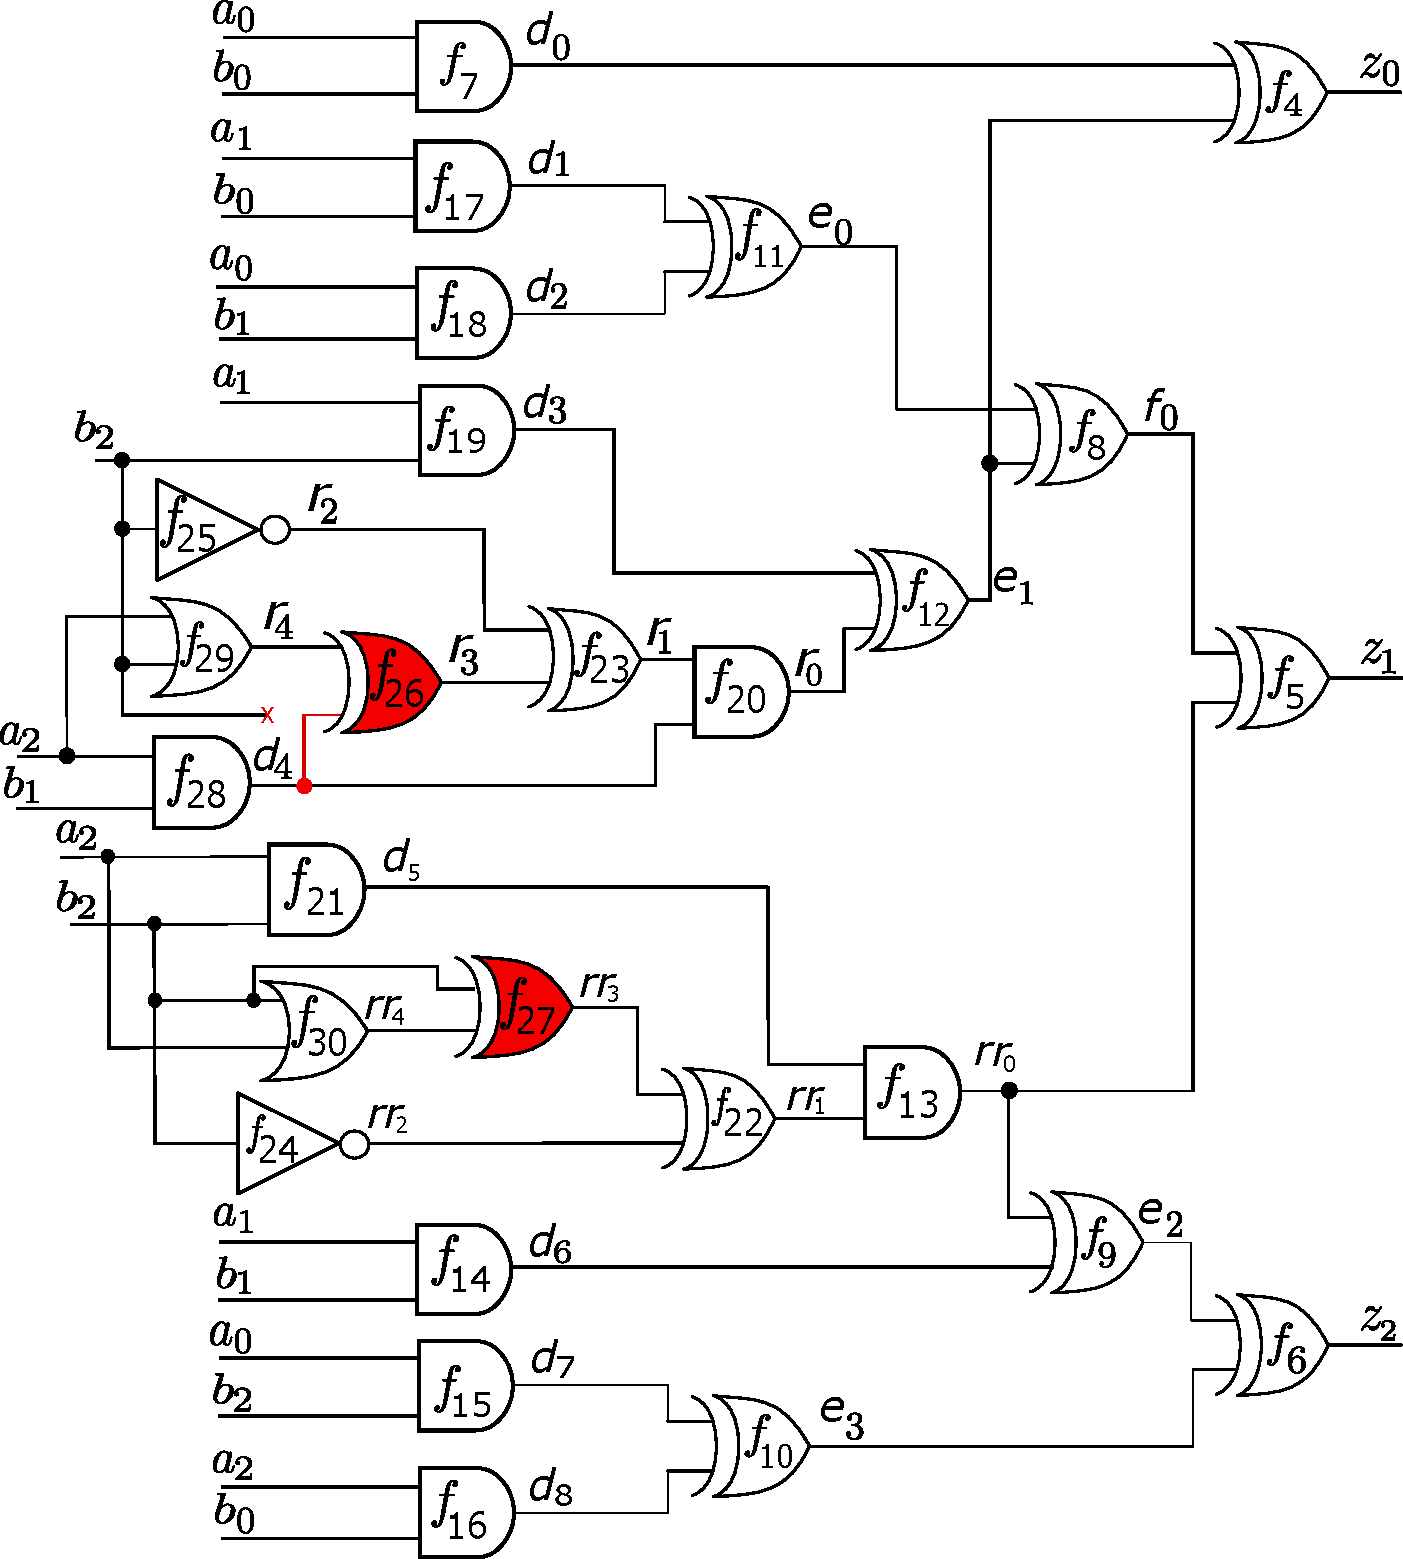
\includegraphics[scale=0.24]{mas_3_ddc_mfr_a.pdf}
\caption*{A faulty implementation of a 3-bit ($n$=3) Mastrovito multiplier
% ($n$=3) with gate replacement bugs introduced at nets $d_5$ (AND replaced with an OR) and $d_2$ (AND replaced with an XOR), and a wire replacement bug at net $e_0$ (input shorted to $d_0$ instead of $d_1$).
}
\end{figure}
\end{frame}

\begin{frame}{\large MFR example: Word-level representation}
\begin{figure}[hbt]
\centering
    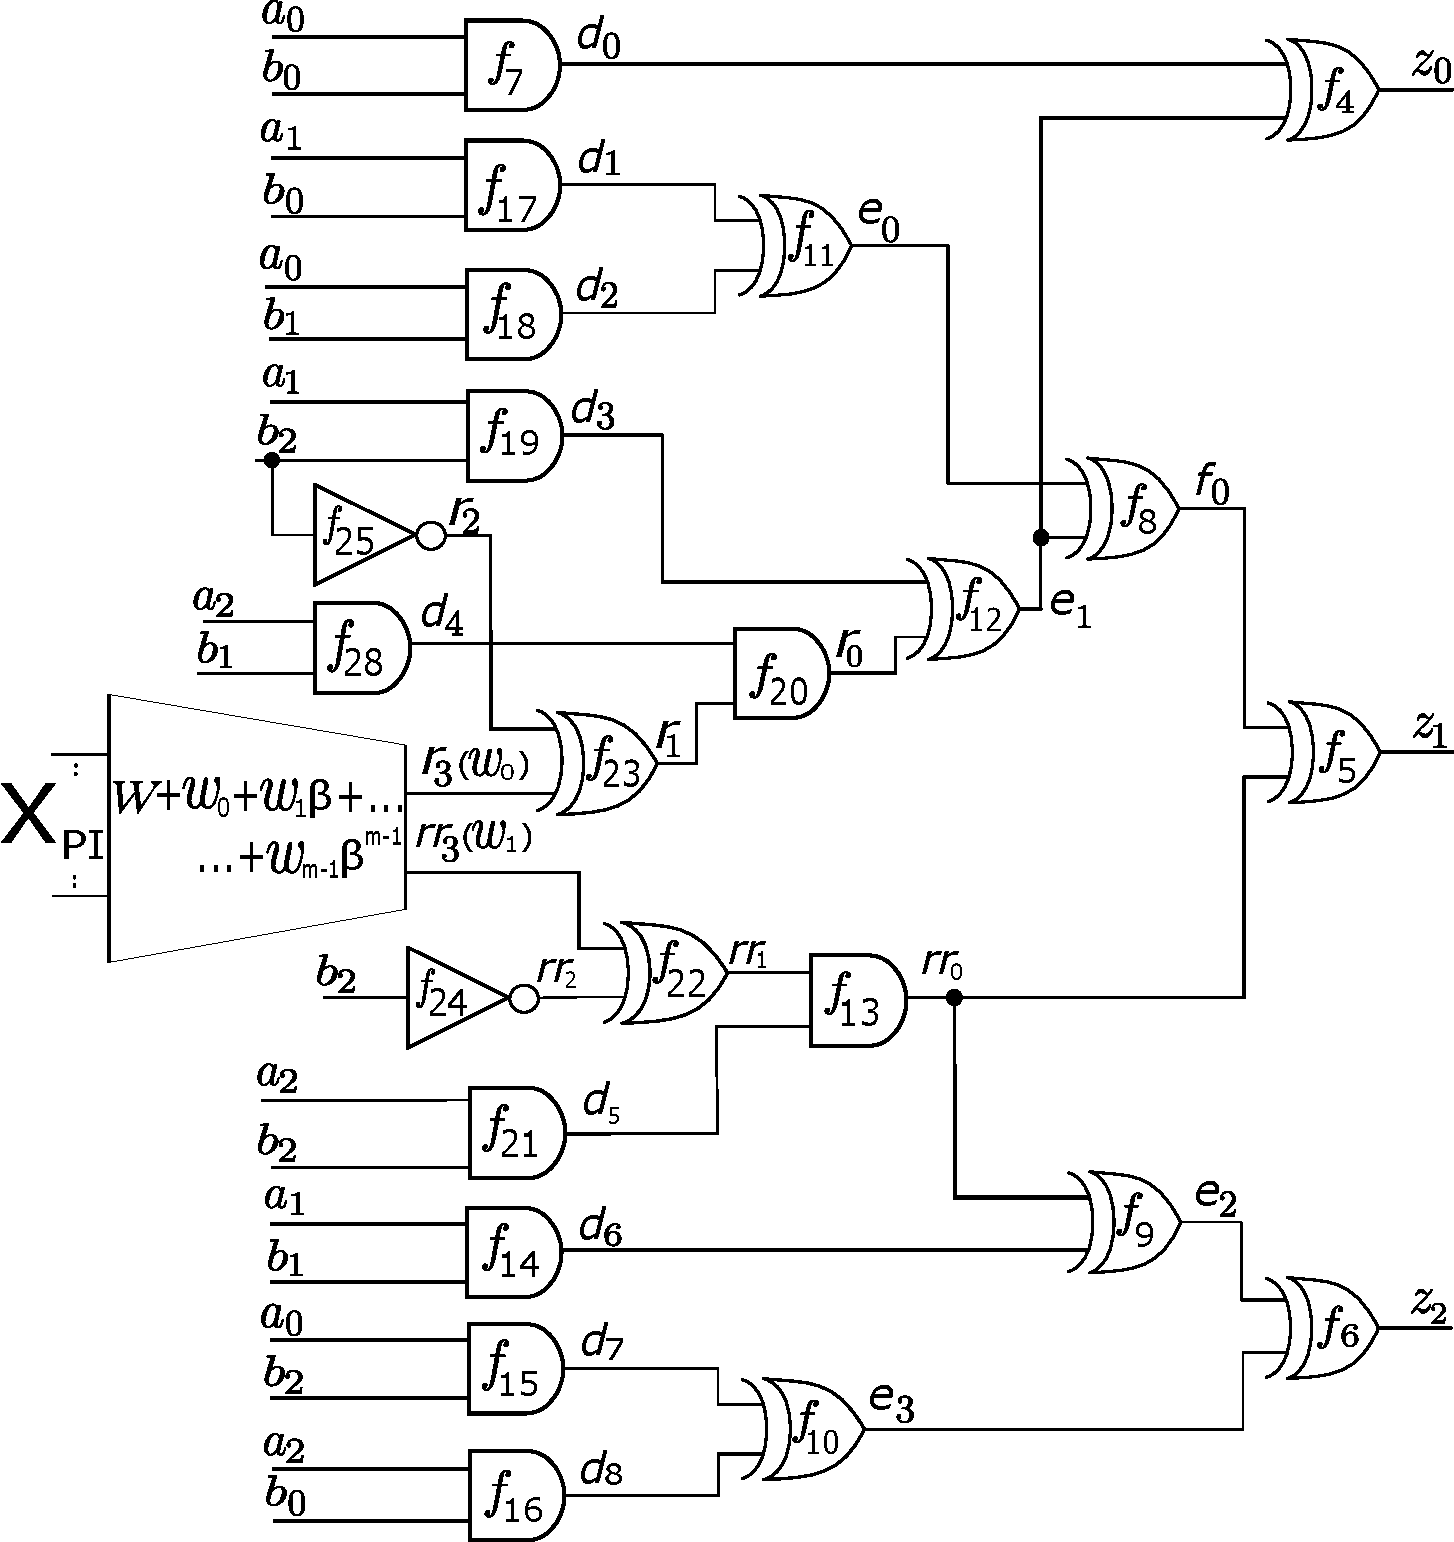
\includegraphics[scale = 0.24]{mas_3_ddc_mfr_b.pdf}
    \caption*{
    Patch function modeled as a 2-bit-vector word ($m$=2) $W=\{r_3,rr_3\} = r_3+\be rr_3$ ($w_0=r_3, w_1=rr_3$).}
    \label{fig:mas_bug_Wb}
\end{figure}
\end{frame}

\begin{frame}{\large Mathematical Challenge: Picking $P_k(x)$}
\bi 

	\item Need to represent and manipulate circuit polynomials and the patch function polynomials
		in one unified domain (composite field)
	% \bi
	% 	\item How to relate algebraic numbers of lower field to algebraic numbers of higher fields?
	% \ei
	\vspace{0.1in}
	\item Selecting arbitrary $P_k(x)$ leads to erroneous results 
	\vspace{0.1in}
	\item Solved using Univariate Polynomial Factorization

\ei
\end{frame}


\begin{frame}{\large MFR Notations: Composite Field}
\bi
	\item For a given circuit with data-path size $n$
	\bi
		\item Polynomials modeled over $R=\Fkn[Z,A,x_1,\dots,x_d]$
		\bi
			\item $\{x_1, \dots$ $, x_d\}$ are all the bit-level variables (nets) in the circuit
			\item $Z$ and $A$ are the word-level output and input, respectively
		\ei
		\item $\Fkn$ is constructed as $\Fkn = \Ftwo[X]\pmod{P_n(X)}$
		\bi
			\item $P_n(X) \in \F_2[X]$ is a given degree-$n$ primitive polynomial; $P_n(\ga) =0$ 
			% [$\ga$ as one of its root].
		\ei
		\item  The word-level polynomials for $Z,A$ are modeled as:
		\bi
			\item $f_z: Z + \sum_{i=0}^{n-1}\ga^iz_i;f_a: A + \sum_{i=0}^{n-1}\ga^ia_i;$ 
		\ei
	\ei 
	\item Patch $W$ for $m$ targets is computed as a polynomial function in the field $\Fkm$
	\bi
		\item $\Fkm$ is constructed as $\Fkm = \Ftwo[X]\pmod{P_m(X)}$
		\bi
			\item We select a degree-$m$ primitive polynomial $P_m(X)\in \F_2[X]$; $P_m(\be) =0$ 
			% [$\be$ as one of its root].
		\ei
		\item  The word-level polynomial for $W$ is modeled as:
		\bi
			\item $f_w: W + \sum_{i=0}^{m-1}\be^iw_i$
			\item $\{w_0,\dots,w_{m-1}\} \subset \{x_1,\dots,x_d\}$
		\ei
	\ei
\ei
\end{frame}

\begin{frame}{\large MFR Notations: Composite Field}
\bi
	\item Determine the smallest single field ($\Fkk$) to operate both circuit ($\Fkn$) and patch ($\Fkm$)
	\vspace{0.1in}
	\item Smallest $k$ is $LCM(n,m)$
	\bi
		\item $\Fkk \supset \Fkn$ and $\Fkk \supset \Fkm$
		\item $\Fkk$ is constructed as $\Fkk = \Ftwo[X]\pmod{P_k(X)}$
		\bi
			\item $P_k(X)$ is a degree-$k$ primitive polynomial; $P_k(\al) =0$ 
		\ei
	\ei
	\vspace{0.1in}
	\item  Mathematical challenge: Given $P_n(X)$ and $P_m(X)$, compute $P_k(X)$ such that
	$P_n(\ga)= P_m(\be)=P_k(\al)=0$
	\vspace{0.1in}
	\bi
		\item $\ga = \al^{(2^k-1)/(2^n-1)} = \al^{\lambda}$
		\item $\be = \al^{(2^k-1)/(2^m-1)} = \al^{\mu}$
	\ei
	\vspace{0.1in}
	\item Solved using factorization of univariate polynomials over finite fields
\ei

\end{frame}

\begin{frame}{\large MFR Notations: Univariate Polynomial factorization (UPF) }
\bi
	\item Given a monic univariate polynomial $f \in \F_q[X]$, where $\F_q$ is any finite field
	\vspace{0.1in}
	\bi 
		\item Find a complete factorization $f = f_1^{e_1}\cdot f_2^{e_2}\cdots f_l^{e_l}$ 
		\bi
			\item Where $f_1, f_2,\dots, f_l$ are pairwise distinct monic 
			irreducible polynomials in $\F_q[X]$ and $e_1,\dots,e_l$ are positive integers.
		\ei
	\ei
	\vspace{0.1in}
	% \item We employ existing implementation of UPF from computer algebra tool {\it SINGULAR} 
\ei
\end{frame}

\begin{frame}{\large MFR Notations: Finding Primitive Polynomial $P_k(X)$}
\bi
	\item Obtain UPFs of $P_n(X^{\lambda})$ and $P_m(X^{\mu})$
	\bi
		\item Coefficients will be in $\Ftwo$ and degrees will be less than $\lambda$ and $\mu$, respectively.
		\bi
			\item $P_n(X^{\lambda})=P_{n1}^{a1}\cdot P_{n2}^{a2}\cdots P_{nl}^{al}$, and 
			\item $P_m(X^{\mu}) = P_{m1}^{b1}\cdot P_{m2}^{b2}\cdots P_{mg}^{bg}$
		\ei
	\ei
	\vspace{0.1in}
	\item Conjecture: $\exists P_{ni}(X) \in \{P_{n1}, P_{n2},\dots ,P_{nl}\}$ and $\exists P_{mj}(X) \in \{P_{m1}, P_{m2},\dots ,P_{mg}\}$, such that:
	\bi
		\item $P_k(X) = P_{ni}(X)=P_{mj}(X)$,
		\item $P_{k}(X)$ is a degree-$k$ primitive polynomial in $\F_2[X]$ such that $P_k(\al)=0$
	\ei
\ei
\end{frame}


\begin{frame}{\large MFR Application: Word-level Formulation}
\bi
	\item Update ring properties 
	\bi
		\item $R=\F_q[x_1,\dots,x_d,Z,A,W]$
		\item Modify RTTO $>$ to place the target $W$ before the lowest indexed target $e_0$
		\bi
			\item $\{Z\}>\{A>B\}>\{z_0>z_1>z_2\}>\{f_0>e_2>e_3\}>\{{\bf{W}}>e_0>e_1>d_5>d_6>d_7>d_8\}>
				\{d_0>d_1>d_2>d_3>d_4\}>\{a_0>a_1>a_2>b_0>b_1>b_2\}.$
		\ei
	\ei
	\vspace{0.1in}
	\item Update polynomial set $F$ to $F'$:
	\bi
		\item Delete polynomials for $w_i$'s
		\item Delete polynomials in the transitive fan-in of $w_i$'s only
		\item Transitive fan-outs of $w_i$'s need to be replaced with their equivalent 
		word-level representations in terms of $W$
		\item Add $f_w: W + \sum_{i=0}^{m-1}\be^iw_i$
	\ei

\ei
\end{frame}

\begin{frame}{\large MFR Application: Computing $P_k(X)$}
\bi
	\item Composite field: $k=LCM(2,3)=6$
	\vspace{0.1in}
	\bi
		\item $UPF(P_3(X^9)) = \{{\bf X^6+X^4+X^3+X+1},X^6+X^4+X^2+X+1,{\bf X^6+X^5+1}, X^6+X^5+X^2+X+1\}$
		\vspace{0.1in}
		\item $UPF(P_2(X^{21})) = \{{\bf X^6+X^4+X^3+X+1}, {\bf X^6+X^5+1}, X^6+X^3+1, X^6+X^5+X^2+X+1, X^6+X^5+X^3+X^2+1, X^6+X+1, X^6+X^5+X^4+X+1 \}$
		\vspace{0.1in}
		\item We will pick $P_6(X)=X^6+X^4+X^3+X+1$ as the primitive polynomial to setup the unified framework.
	\ei
\ei
\end{frame}

\begin{frame}{\large MFR Notations: Incorrect Primitive Polynomial}
\bi
	\item Note that if we incorrectly choose $P_k(X)=X^6+X^3+1$
	\item For its root $\al$, we have
	\begin{center}
		$\al^6+\al^3+1=0$\\
		$(\al^3)(\al^6+\al^3+1)=0$ (multilying by $\al^3$)\\
		$\al^9+\al^6+\al^3=0$\\
		$\ga+1=0$\label{ga_val}
	\end{center}
	\item But we have $\ga=\al^9$
	\item Selecting arbitrary $P_k(X)$ leads to erroneous results
\ei
\end{frame}

\begin{frame}{\large MFR Application: Word-level Formulation }
\bi
	\item 2-bit rectification patch over the 3-bit circuit can be performed over the field $\F_{2^6}$
	\bi
		\item Field $\F_{2^6} = \F_2[X]$ (mod $P_6(X)$)
	\ei
	\vspace{0.1in}
	\item Update polynomial set $F$ to $F'$ as:
	\begin{center}
		\begin{align*}
			F'=\{f_1,\dots,f_3,f'_4,f'_5,f_6,f'_7,f'_8,f_9,f_w,f_{11},f_{13}\dots,f_{20}\}
		\end{align*}
		{\small\begin{flalign*}
			f'_4:z_0 + (\be W^2 +\be^2 W) + d_0;     &\quad f'_5:z_1 + f_0 + (W^2+W); \\
			f'_7:f_0 + (\be W^2 +\be^2 W) + e_1;   &\quad f'_8:e_2 + (W^2+W) + d_6; \\
			f_w:W + e_0 + \be d_5;             &\quad \be=\al^{21} ; \ga=\al^9;
		\end{flalign*}}
	\end{center}

\ei
\end{frame}

\begin{frame}{\large MFR Contribution: Rectification Check}
%ATPG V() V() = empty
%we have an algebraic proof which is there in the proposal
\bi
	\item Multi-fix rectification at target $W$
	\vspace{0.1in}
	\bi
		\item Construct the following ideals:
		\bi
			\item {\small $J_i = \langle F'_i\rangle =\{f'_1,\dots,f_w=W+\delta(i),\dots,f'_s\}$}
				:$1 \leq i \leq 2^m$, $\delta(0)=0, \delta(1)=1,\delta(2)=\be,\dots,\delta(2^m)= \be^{2^m-2}$
		\ei
		\vspace{0.1in}
		\item Performing the reductions for all $1 \leq i \leq 2^m$: 
		\bi
			\item $f\xrightarrow{F'_i, F_{0}^{PI}}_+r_i $
		\ei
		\item Let $V_{\Fq}(r_i)$ denote the varieties of the respective $r_i$'s
		\vspace{0.1in}
		\item Multi-fix rectification exists at target $W$: \\ 
				\centering
				{\bf if and only if} $\bigcup\limits_{i=1}^{2^m}V_{\Fq}(r_i) = \Fq^{|X_{PI}|} = V(J_0^{PI})$
	\ei
\ei
\end{frame}

\begin{frame}{\large MFR Application: Rectification Check}
\bi
	\item Constructing the $J_i$ ideals:
	\bi
		\item {\small$J_1 = \langle F'_1\rangle$, where $F'_1[f_w]=W+\delta(1)=W$},
		\item {\small$J_2 = \langle F'_2\rangle$, where $F'_2[f_w]=W+\delta(2)=W+1$},
		\item {\small$J_3 = \langle F'_3\rangle$, where $F'_3[f_w]=W+\delta(3)=W+\be$},
		\item {\small$J_4 = \langle F'_4\rangle$, where $F'_4[f_w]=W+\delta(4)=W+\be^2$}
	\ei
	\vspace{0.1in}
	\item Reducing the specification $f: Z+A\cdot B$ modulo these ideals, we get:
	\bi
		\item $r_1 = f \xrightarrow[]{F'_1,F_{0}^{PI}}_+{a_1b_2\ga^3+a_2b_1\ga^3+\ga^4a_2b_2}$
		\item $r_2 = f \xrightarrow[]{F'_2,F_{0}^{PI}}_+{a_1b_2\ga^3+a_2b_1\ga^3+\ga^4a_2b_2+\ga^3}$
		\item $r_3 = f \xrightarrow[]{F'_3,F_{0}^{PI}}_+{a_1b_2\ga^3+a_2b_1\ga^3+\ga^4a_2b_2+\ga^4}$
		\item $r_4 = f \xrightarrow[]{F'_4,F_{0}^{PI}}_+{a_1b_2\ga^3+a_2b_1\ga^3+\ga^4a_2b_2+\ga^6}$
	\ei
	\item Computing $GB(r_1\cdot r_2 \cdot r_3 \cdot r_4, F_{0}^{PI})=F_{0}^{PI}$
	\item Target $W$ with nets $e_0$ and $d_5$ admits MFR
\ei
\end{frame}


% \begin{frame}{\large MFR Pseudocode}
% \begin{figure}[hbt]
% \centering
%     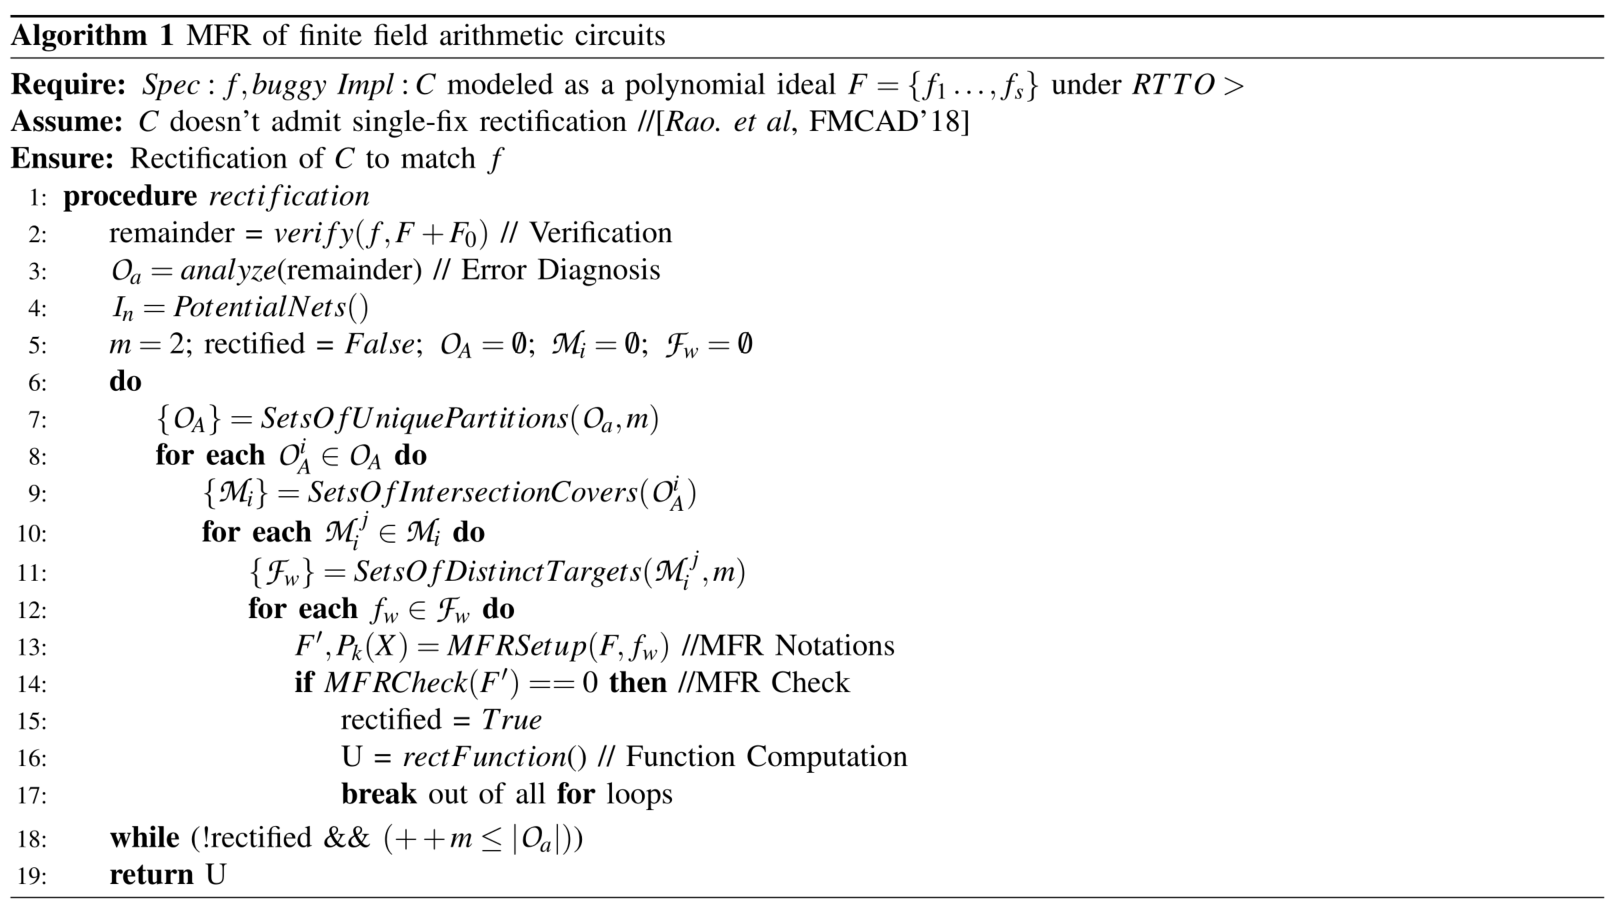
\includegraphics[scale = 0.43]{algo.png}
% \end{figure}
% \end{frame}

% \begin{frame}{\large Research Objective: Synthesis of Rectification Function}
% \begin{figure}[hbt]
%     \begin{center}
%     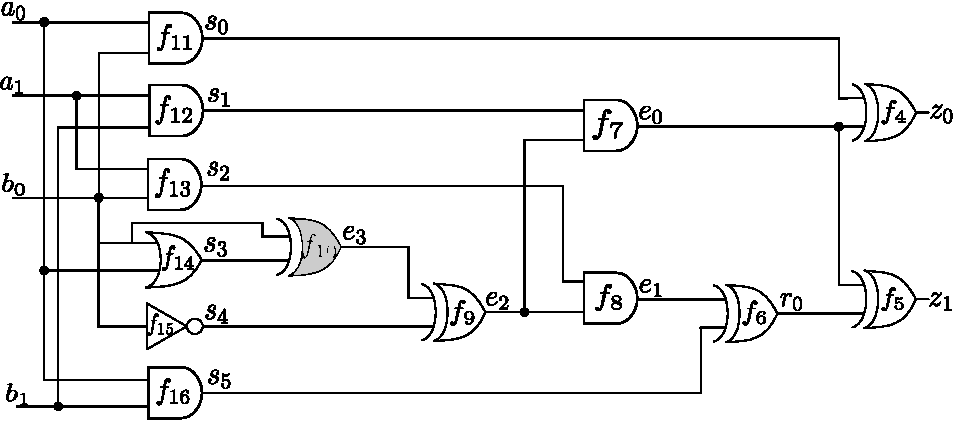
\includegraphics[scale = 0.7]{mas_red_bug-eps-converted-to.pdf}
%     \end{center}
% %    \vspace{-4ex}
%     \caption*{\small A 2-bit buggy modulo
%       multiplier implementation. 
%     %   with the bug at
%     % net $e_3$. A correct implementation will have an AND gate at $e_3$,
%     % which has been replaced by an XOR gate.
%     }
%     \label{fig:mas_both}
% \end{figure}
% \end{frame}

% \begin{frame}{\large Research Objective: Exploring don't cares}
% \begin{small}
% $r \in \langle h_{10},f_{11},f_{12},f_{13},f_{14},f_{15},f_{16}\rangle
%   + \langle F_{0}^{PI}\rangle$ \\
% $r = U\cdot h_{10} + h_{11}f_{11} + h_{12}f_{12}+h_{13}f_{13}+h_{14}f_{14}+h_{15}f_{15}+h_{16}f_{16}$ \\
% $U = b_0$; $U^1 = a_1*b_0$; $U^2 = a_1*b_1*b_0+a_1*b_1+a_1$;
% \end{small}
% {\tiny 
% \begin{table}[ht]
%     \centering
%     \begin{tabular}{|c|c|c|c|c|} \hline
%       $\{a_0a_1b_0b_1\}$ & $h_{10}$ & $U$ & ${U^1}$ & ${U^2}$ \\ \hline
% 		0000 & 0     & 0 & 0 & 0 \\ \hline
% 		0001 & 0     & 0 & 0 & 0 \\ \hline
% 		0010 & 0     & 1 & 0 & 0 \\ \hline
% 		0011 & 0     & 1 & 0 & 0 \\ \hline
% 		0100 & 0     & 0 & 0 & 1 \\ \hline
% {\it    0101}& (x+1) & 0 & 0 & 0 \\ \hline
% {\bf    0110}& (x)   & 1 & 1 & 1 \\ \hline
% {\bf	0111}& 1     & 1 & 1 & 1 \\ \hline
% 		1000 & 0     & 0 & 0 & 0 \\ \hline
% 		1001 & 0     & 0 & 0 & 0 \\ \hline
% 		1010 & 0     & 1 & 0 & 0 \\ \hline
% 		1011 & 0     & 1 & 0 & 0 \\ \hline
% 		1100 & 0     & 0 & 0 & 1 \\ \hline
% {\it    1101}& (x+1) & 0 & 0 & 0 \\ \hline
% {\bf    1110}& (x)   & 1 & 1 & 1 \\ \hline
% {\bf    1111}& 1     & 1 & 1 & 1 \\ \hline
%     \end{tabular}
%     \caption{Evaluating quotient and rectification solutions}
% \end{table}}

% \bi
% 	\item Challenge: Word-level formulation of don't cares
% \ei

% \end{frame}

% \begin{frame}{\large Research Objective: Logic optimization using don't cares}
% \bi
% 	\item $h_{10}$ represents the ODCs for the selected target $e_3$
% 	\bi
% 		\item Algorithm to explore don't care setup
% 	\ei
% 	\vspace{0.1in}
% 	\item Logic simplification using permissible functions
% 	\bi
% 		\item {\it Fujita} has an approach using BDDs
% 		\item Investigate the application in algebraic setting
% 	\ei
% \ei
% \end{frame}

